
\documentclass[12pt]{article}
\usepackage[a4paper, margin=.30in]{geometry}
\usepackage{graphicx ,
            wrapfig,
            xcolor, 
            enumerate,
            amsmath,
			fontenc,
			tcolorbox,circuitikz,tikz,bm
            }
			\usepackage{pgfplots}
\pgfplotsset{compat=newest}
\usepgfplotslibrary{fillbetween}
\usepackage{pgfplots}
\newcommand\headerMe[2]{\noindent{}#1\hfill#2}
\renewcommand{\thesection}{\Roman{section}}

\author{Zakaria HAOUZAN}
\date{\today}

\begin{document}
% headers --------------
\headerMe{Matière : Physique-Chimie}{Professeur : Zakaria HAOUZAN}\\
\headerMe{Unité : Mécanique }{Établissement : Lycée SKHOR qualifiant}\\
\headerMe{Niveau : 2BAC-SM-PC}{Heure : 6H}\\

% ------Content ________
\begin{center}

    \Large{Leçon $N^{\circ} 14 $: \color{red}Mouvement de rotation d’un solide autour d’un axe fixe.}
\end{center}

\begin{wrapfigure}[5]{r}{0.3\textwidth}
	\vspace{-1cm}
	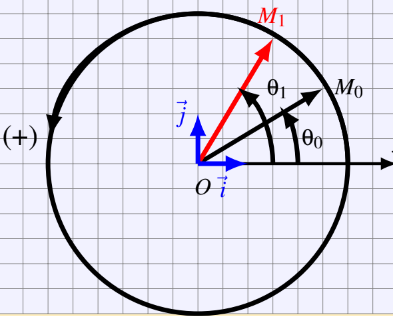
\includegraphics[width=0.3\textwidth]{./img_00.png}
\end{wrapfigure}

\section{Abscisse angulaire - accélération angulaire. }
\subsection{Rappel : }
Un corps solide est en mouvement circulaire autour d'un axe fixe si tous ses points décrivent des trajectoires circulaires
centrées sur cet axe (seuls les points situés sur cet axe sont immobiles).

\subsection{Repérage de la position d'un mobile: }

On repère la position d'un solide en mouvement de rotation autour d'un axe fixe $(\Delta)$ en utilisant l'abscisse curviligne ou bien l'abscisse angulaire.

-abscisse angulaire : $\theta$

-abscisse curviligne : $s$

Relation entre l'abscisse curviligne et l'abscisse angulaire : $s = R.\theta$  R: rayon du cercle ).

\subsection{La vitesse angulaire : }
La vitesse angulaire $\dot\theta$ est la dérivée de l'abscisse angulaire par rapport au temps : $\dot{\theta} = \frac{d\theta}{dt}$ en (rad/s)

La vitesse linéaire : $v$ , est la dérivée de l'abscisse curviligne par rapport au temps : $v = \frac{ds}{dt}$ en (m/s)

Relation entre la vitesse linéaire vitesse angulaire: on a : $s = R.\theta$ par dérivation donc $\frac{ds}{dt} = R . \frac{d{\theta}}{dt}$

alors $v = R.\dot{\theta}$

\subsection{Accélération angulaire et accélération linéaire :}
\begin{wrapfigure}[5]{r}{0.3\textwidth}
	\vspace{-2cm}
	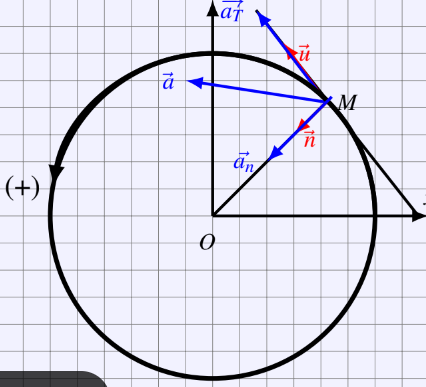
\includegraphics[width=0.3\textwidth]{./img_01.png}
\end{wrapfigure}
L'accélération angulaire est la dérivée de la vitesse angulaire par rapport au temps : $\ddot{\theta}$=$ \frac{d\dot{\theta}}{dt}$ en $(rad/s^2)$

Dans le repère de Frenet le vecteur accélération : $\vec{a} = \vec{a_t} + \vec{a_n}$ possède deux composantes . 

\begin{itemize}
	\item La composante tangentielle : $a_t = \frac{dv}{dt}$ avec $(v = R.\dot{\theta})$  = $R.\ddot{\theta}$

	\item La composante normale : $a_n = \frac{v^2}{R}$ avec $(a_n = R.\dot{\theta}^2)$
\end{itemize}

\section{Le principe fondamentale de la dynamique pour un corps en rotation d'un axe fixe : }

\subsection{Enoncé du PFD: }
La somme des moments des forces extérieures qui s'éxercent sur un solide en rotation autour d’un axe fixe est égale au
moment d’inertie du solide multiplié par son accélération angulaire.

$$\sum{M(\vec{F_{ext}})} = J_{\Delta}.\ddot{\theta}$$

$J_{Delta}$ : Moment d'inertie du corps solide en $(kg.m^2)$

$\ddot{\theta}$ : Accélération angulaire en $(rad/s^2)$


\begin{tcolorbox}

	Si $\ddot{\theta} = 0$, le solide est en mouvement de rotation uniforme ,équation horaire du mouvement est $ \theta $=$\dot{\theta}.t + \theta_0$

	Si $\ddot{\theta} = Cte$, le solide est en mouvement de rotation uniformément varié , l'équation horaire du mouvement est
	$ \dot\theta =  \ddot{\theta}.t + \theta_0$ et l'équation de la vitesse angulaire est: $ \theta =  \frac{1}{2}.\ddot{\theta}.t^2 + \dot\theta.t + \theta_0$
\end{tcolorbox}


\subsection{Expression du moment d'inertie de quelques corps solides:}

\begin{center}

	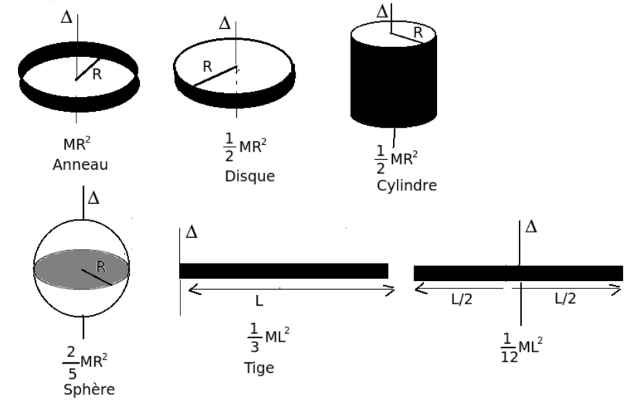
\includegraphics[width=0.6\textwidth]{./img_02.png}
\end{center}



%\begin{wrapfigure}{r}{0.3\textwidth}
	%\vspace{-2cm}
	%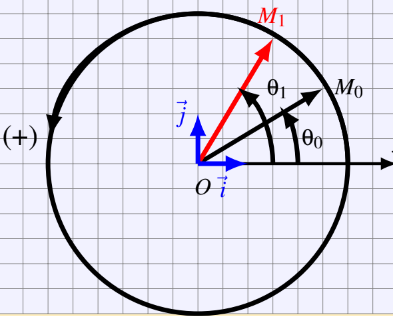
\includegraphics[width=0.3\textwidth]{./img_00.png}
%\end{wrapfigure}

\end{document}

